\section{Dynamical Variational AutoEncoders - Experiments}\label{DVAEs and SDEs}

%
% ------  DKF
%

\begin{frame}{DKF - Toy training - Loss}
    \begin{itemize}
        \item \textbf{Posterior collapse !}
        \item Need $\beta$ schedule (weight between reconstruction loss and $\mathbb{KL}$)
    \end{itemize}
    \begin{center}
        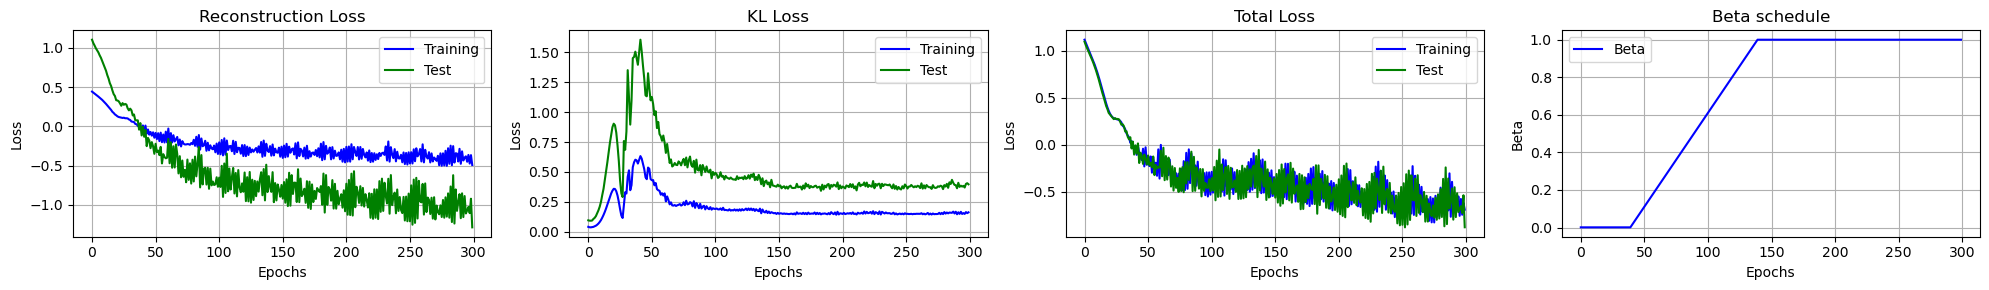
\includegraphics[width=1.0\textwidth]{/home/benjamin/Folders_Python/MVA/MVA_Stage/images/dkf_loss.png}
    \end{center}
    % \caption{DKF Loss}
\end{frame}

\begin{frame}{DKF - Toy training - Generations}
    \begin{center}
    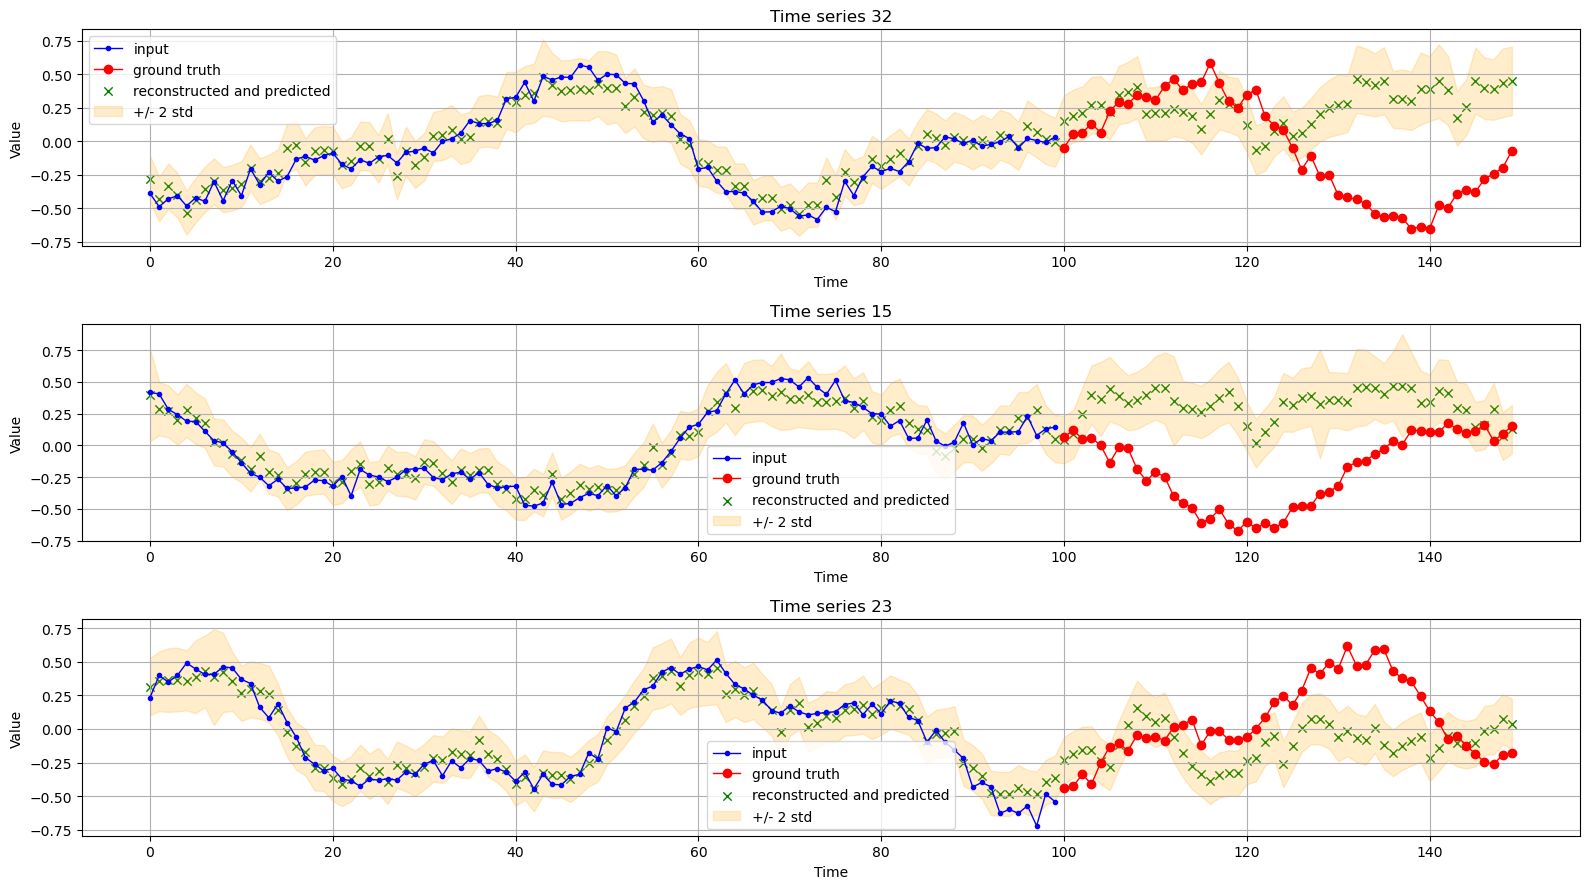
\includegraphics[width=0.8\textwidth]{/home/benjamin/Folders_Python/MVA/MVA_Stage/images/dkf_preds_gens.png}
    % \caption{DKF Predictions}
    \end{center}
\end{frame}

%
% ---- vrnn
%


\begin{frame}{VRNN - Toy training - Loss}
    \begin{itemize}
        \item No posterior collapse
        \item Shorter toy time series to reduce training time
    \end{itemize}
    \begin{center}
        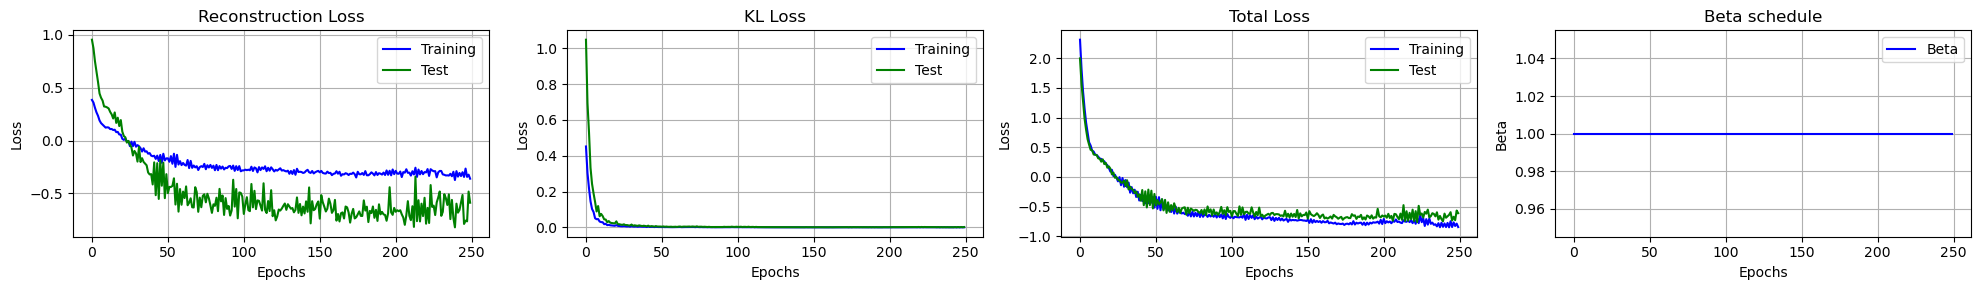
\includegraphics[width=1.0\textwidth]{/home/benjamin/Folders_Python/MVA/MVA_Stage/images/vrnn_loss.png}
    \end{center}
    % \caption{VRNN Loss}
\end{frame}

\begin{frame}{VRNN - Toy training - Generation}
    \begin{center}
    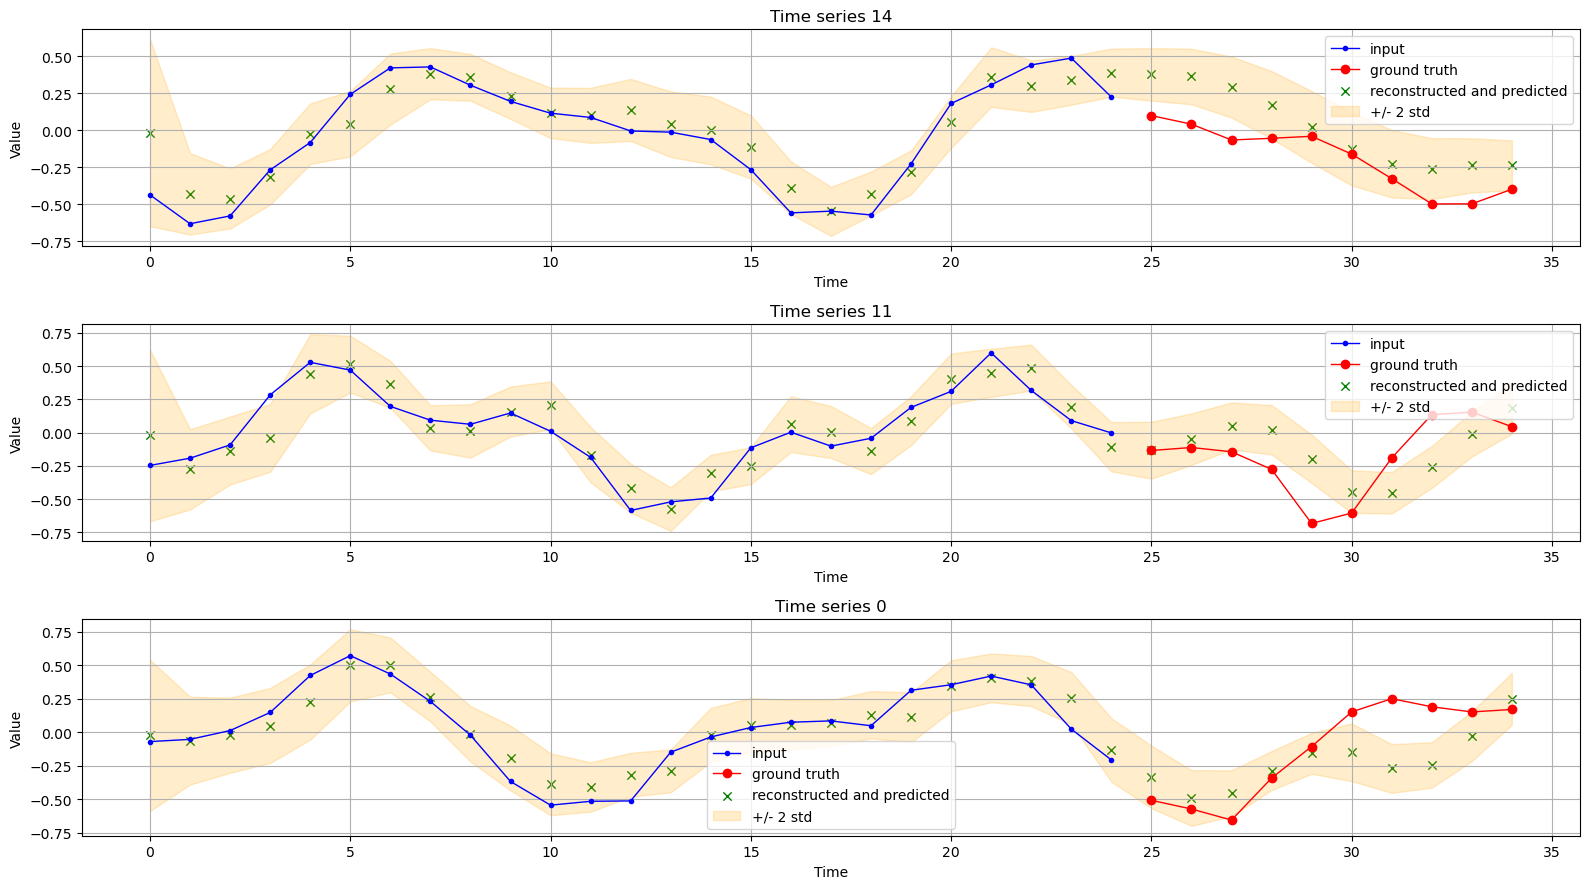
\includegraphics[width=0.6\textwidth]{/home/benjamin/Folders_Python/MVA/MVA_Stage/images/vrnn_preds.png}
    % \caption{VRNN Predictions}
    \end{center}
\end{frame}


\begin{frame}{Sprites dataset}
    \begin{itemize}
        \item Synthetic cartoon characters dataset from \cite{li_disentangled_2018}
        \item RGB images $64 \times 64 \times 3$. 
        \item Each character has 
        \begin{itemize}
            \item 4 attributes (hair, shoes, top cloth, bottom cloth) with 6 possibles values each
            \item 3 possible poses (left, front, right) 
        \end{itemize}
        \item Motion accross time : 3 possible actions (walk, spell, slash) accross 8 consecutive frames.
    \end{itemize}
    \begin{figure}[H]
        \centering
        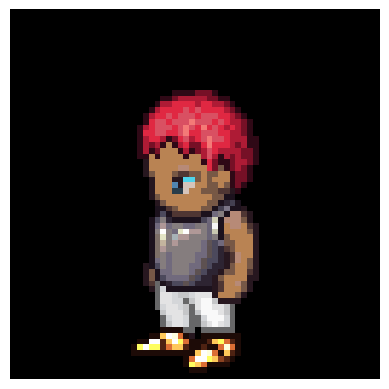
\includegraphics[width=0.2\textwidth]{/home/benjamin/Folders_Python/MVA/MVA_Stage/images/one_sprite.png}
        \caption{One sprite}
        \label{fig:One sprite}
    \end{figure}
\end{frame}
\begin{frame}{Sprites series}
    \begin{figure}[H]
        \centering
        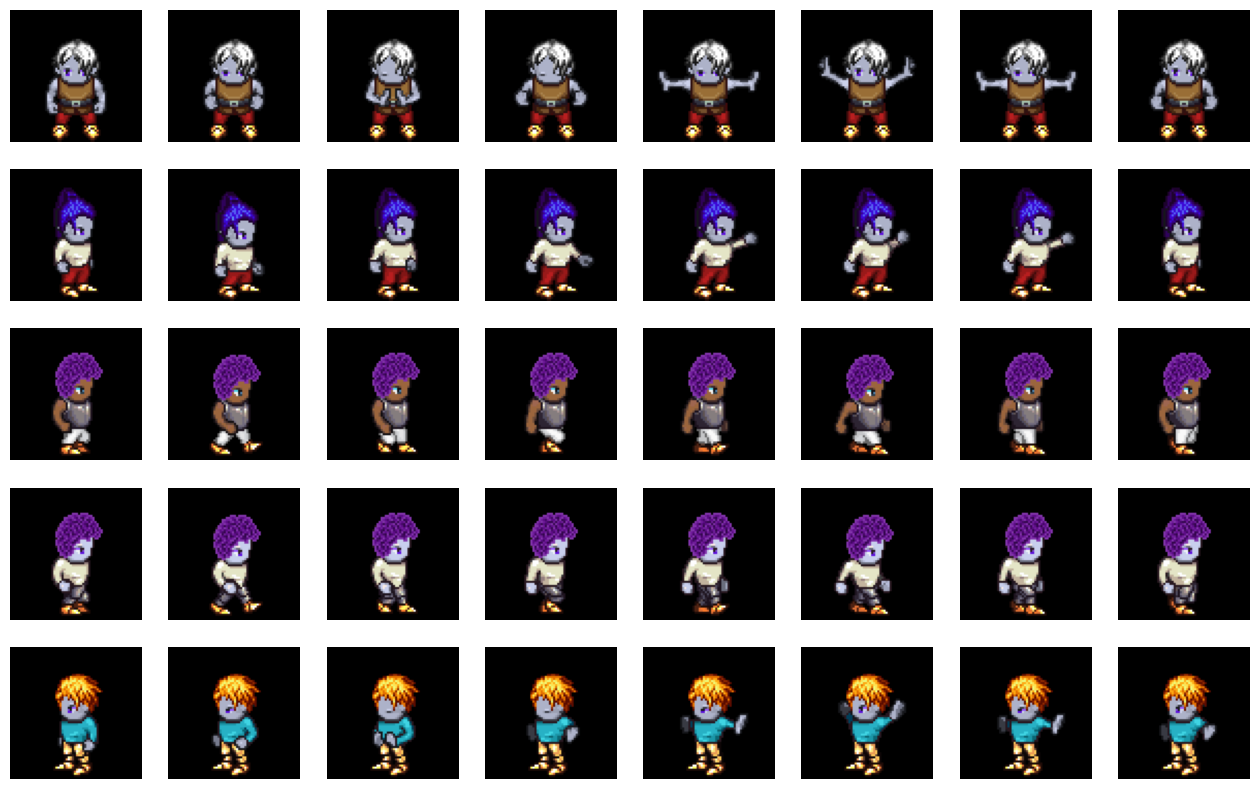
\includegraphics[width=0.7\textwidth]{/home/benjamin/Folders_Python/MVA/MVA_Stage/images/samples_sprites_series.png}
        \caption{sprite series}
        \label{fig:sprite series}
    \end{figure}
\end{frame}

\begin{frame}{VRNN Reconstruction on Sprites}
    \begin{figure}[H]
    \centering
    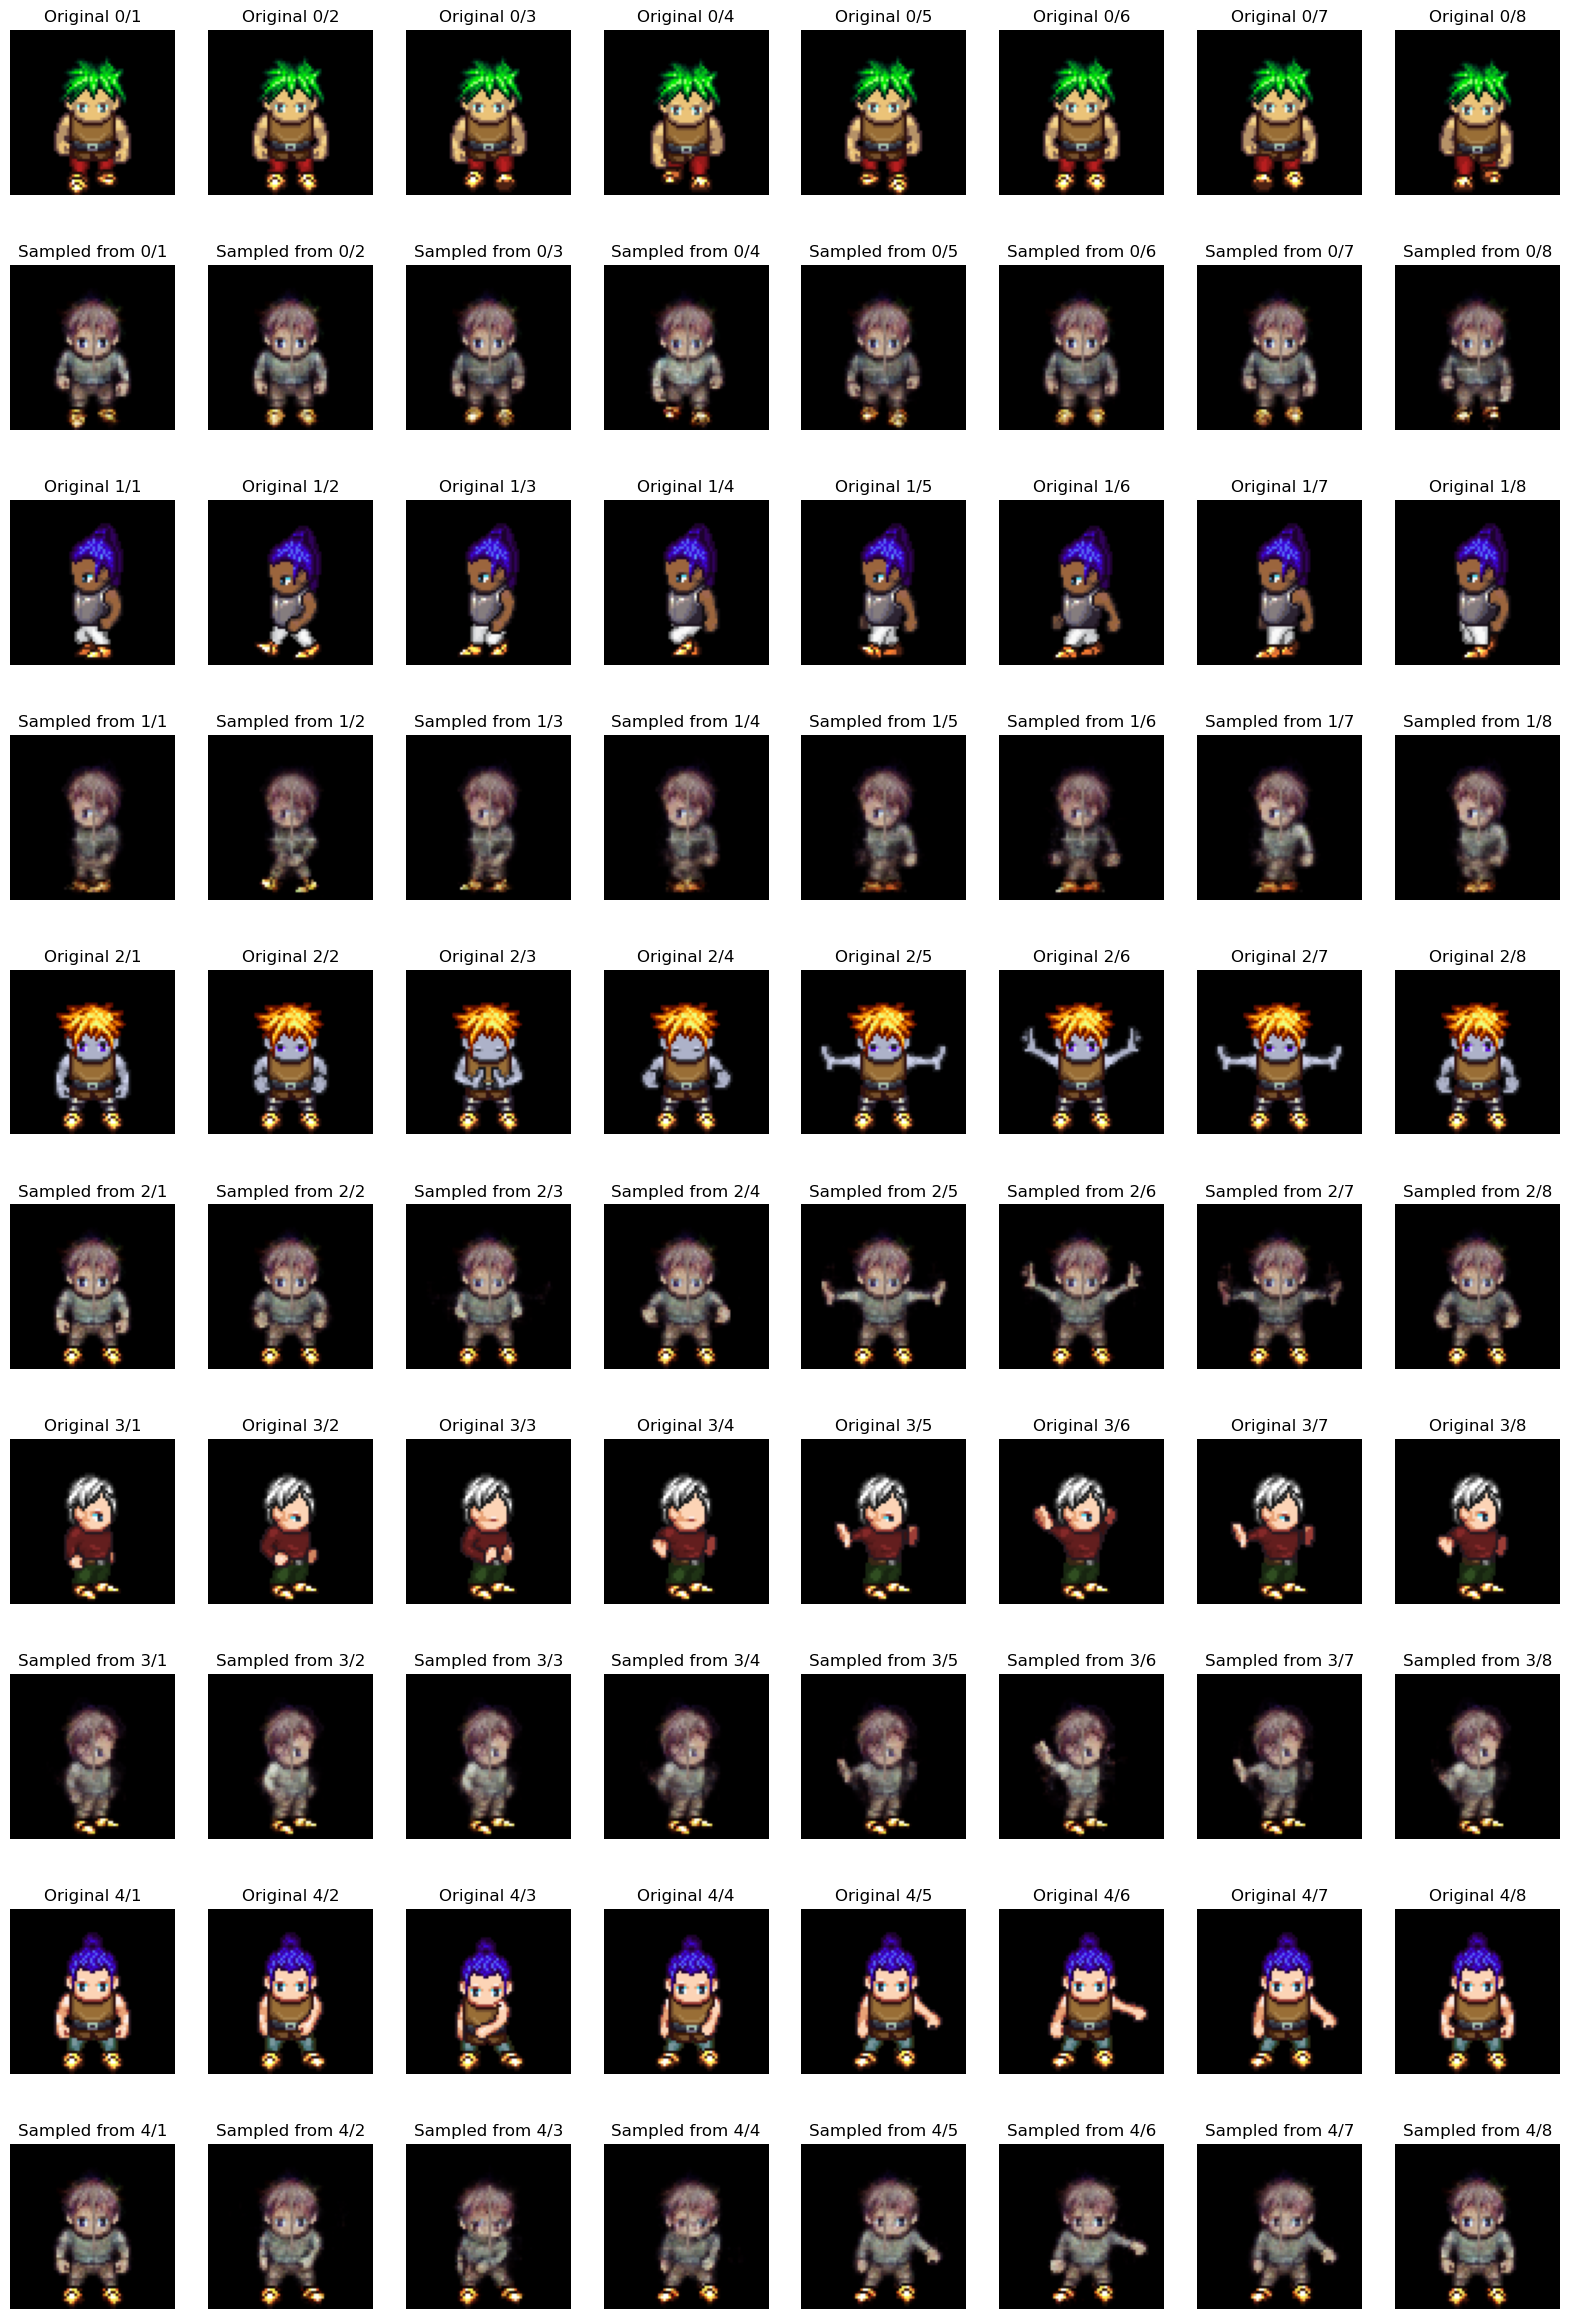
\includegraphics[width=0.6\textwidth]{/home/benjamin/Folders_Python/MVA/MVA_Stage/images/vrnn_sprites_reconstruction.png}
    \caption{VRNN Sprites reconstruction}
    \label{fig:VRNN Sprites reconstruction}
\end{figure}
\end{frame}

\begin{frame}{VRNN Generation}
    \begin{figure}[H]
        \centering
        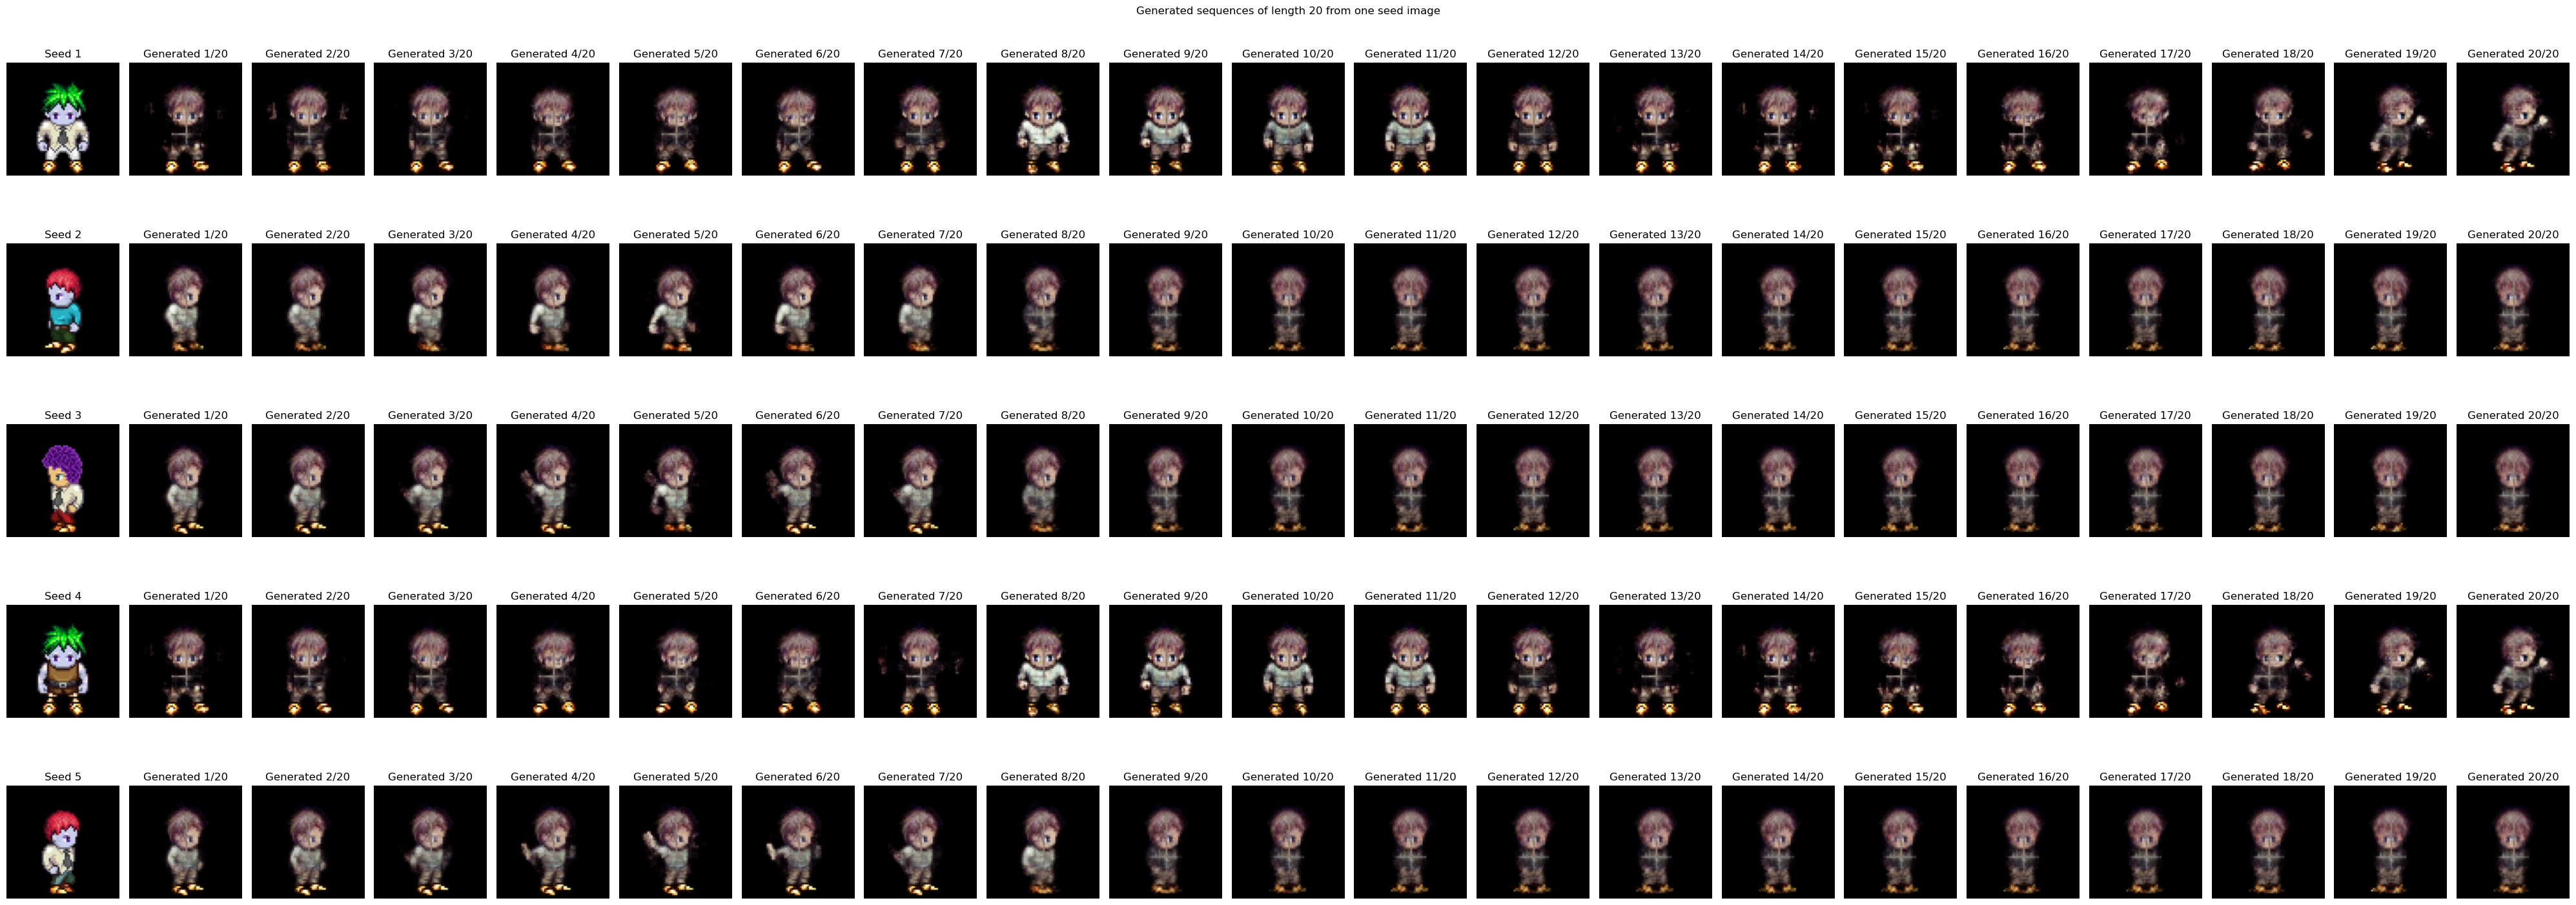
\includegraphics[width=1.1\textwidth]{/home/benjamin/Folders_Python/MVA/MVA_Stage/images/vrnn_sprites_generation.png}
        \caption{VRNN Sprites generation}
        \label{fig:sprite generation}
    \end{figure}
\end{frame}


\begin{frame}{GPVAE - Toy training - Loss}
    $D_x = 4$, $D_y=8$ RBF kernels with decreasing lenghtscales.
    \begin{center}
    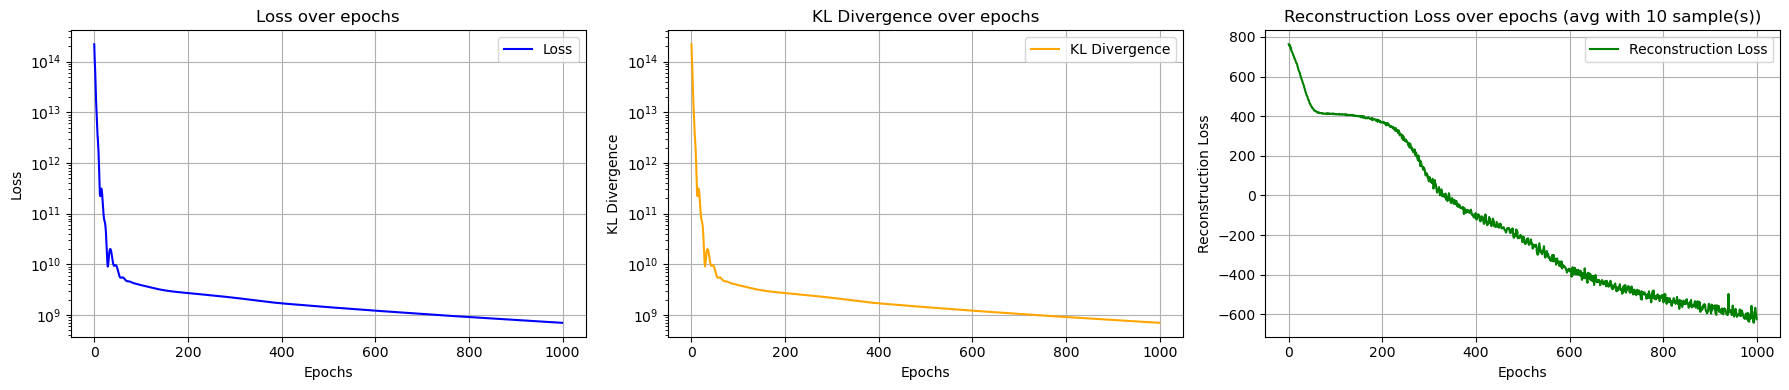
\includegraphics[width=1.0\textwidth]{/home/benjamin/Folders_Python/MVA/MVA_Stage/images/gpvae_loss.png}
    \end{center}
    % \caption{GPVAE Loss}
\end{frame}

\begin{frame}{GPVAE - Toy training - Generations}
    \begin{center}
    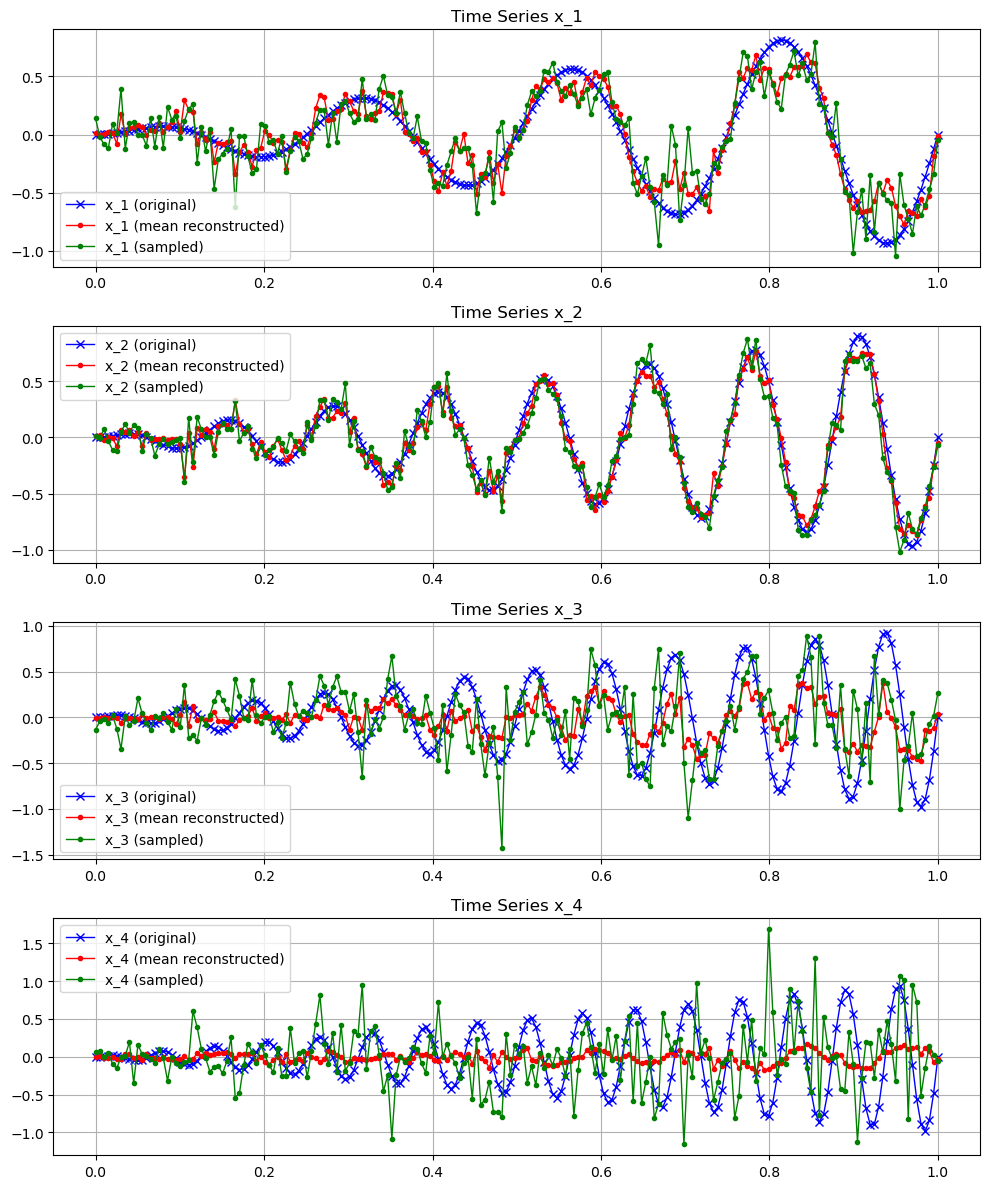
\includegraphics[width=0.4\textwidth]{/home/benjamin/Folders_Python/MVA/MVA_Stage/images/gpvae_preds.png}
    % \caption{GPVAE Predictions}
    \end{center}
\end{frame}

\begin{frame}{GPVAE - Sprites Reconstruction - 1}
    \begin{figure}[H]
    \centering
    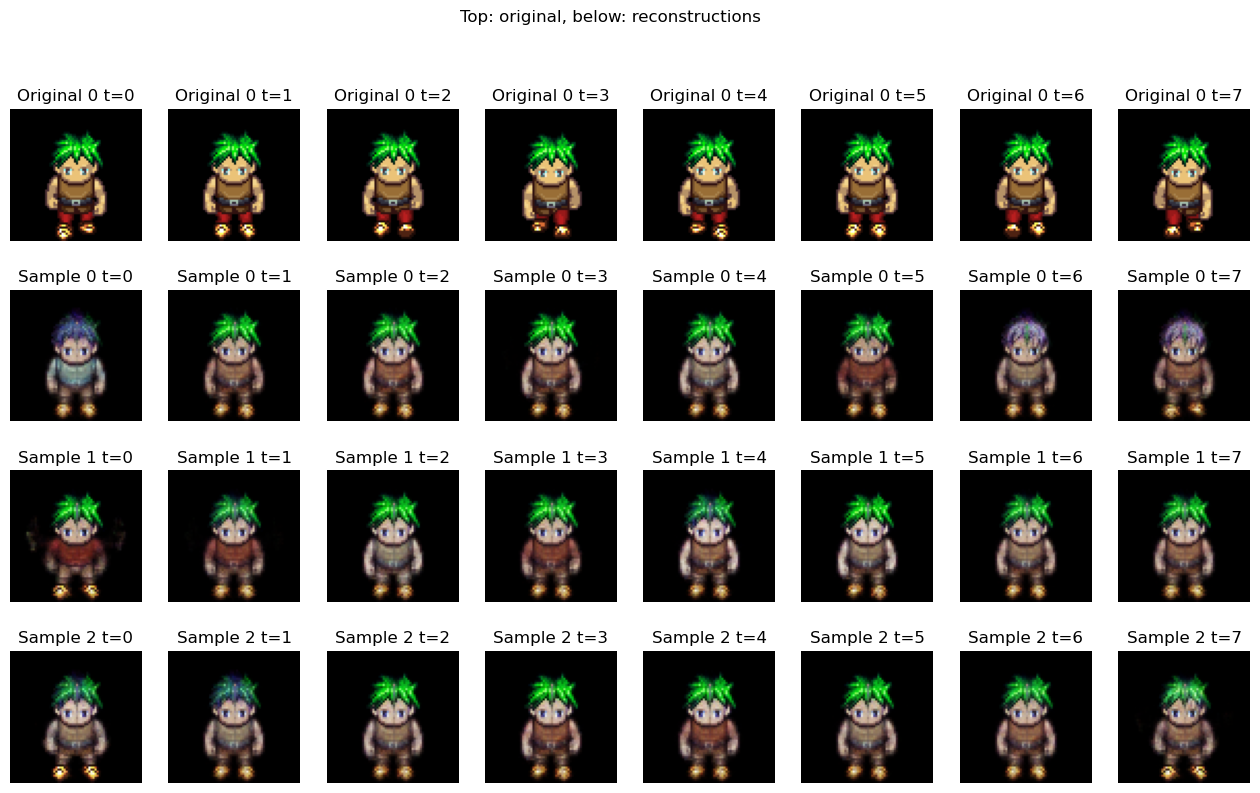
\includegraphics[width=0.7\textwidth]{/home/benjamin/Folders_Python/MVA/MVA_Stage/images/gpvae_reco_01.png}
    \caption{GPVAE Sprites reconstruction 1}
    \label{fig:GPVAE Sprites reconstruction 1}
\end{figure}
\end{frame}

\begin{frame}{GPVAE - Sprites Reconstruction - 2}
\begin{figure}[H]
    \centering
    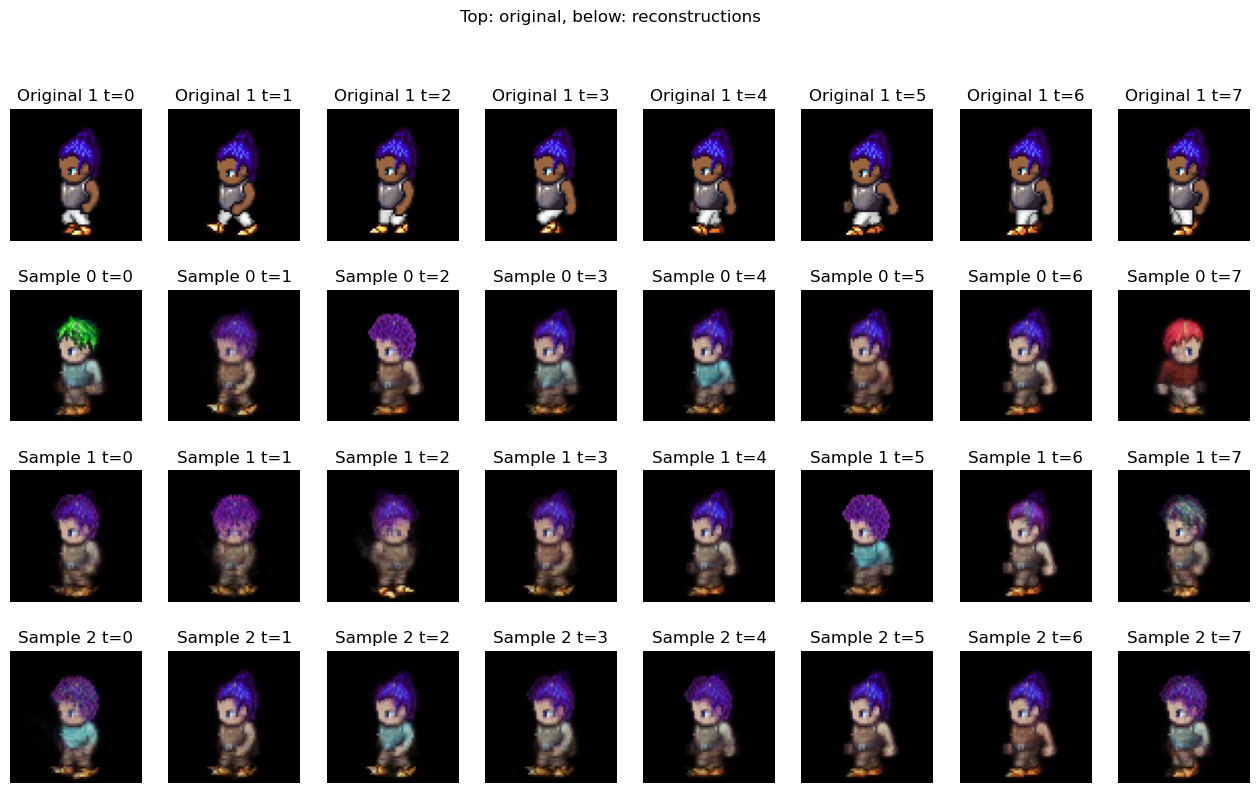
\includegraphics[width=0.7\textwidth]{/home/benjamin/Folders_Python/MVA/MVA_Stage/images/gpvae_reco_02.png}
    \caption{GPVAE Sprites reconstruction 2}
    \label{fig:GPVAE Sprites reconstruction 2}
\end{figure}
\end{frame}

\begin{frame}{GPVAE - Sprites Reconstruction - 1}
\begin{figure}[H]
    \centering
    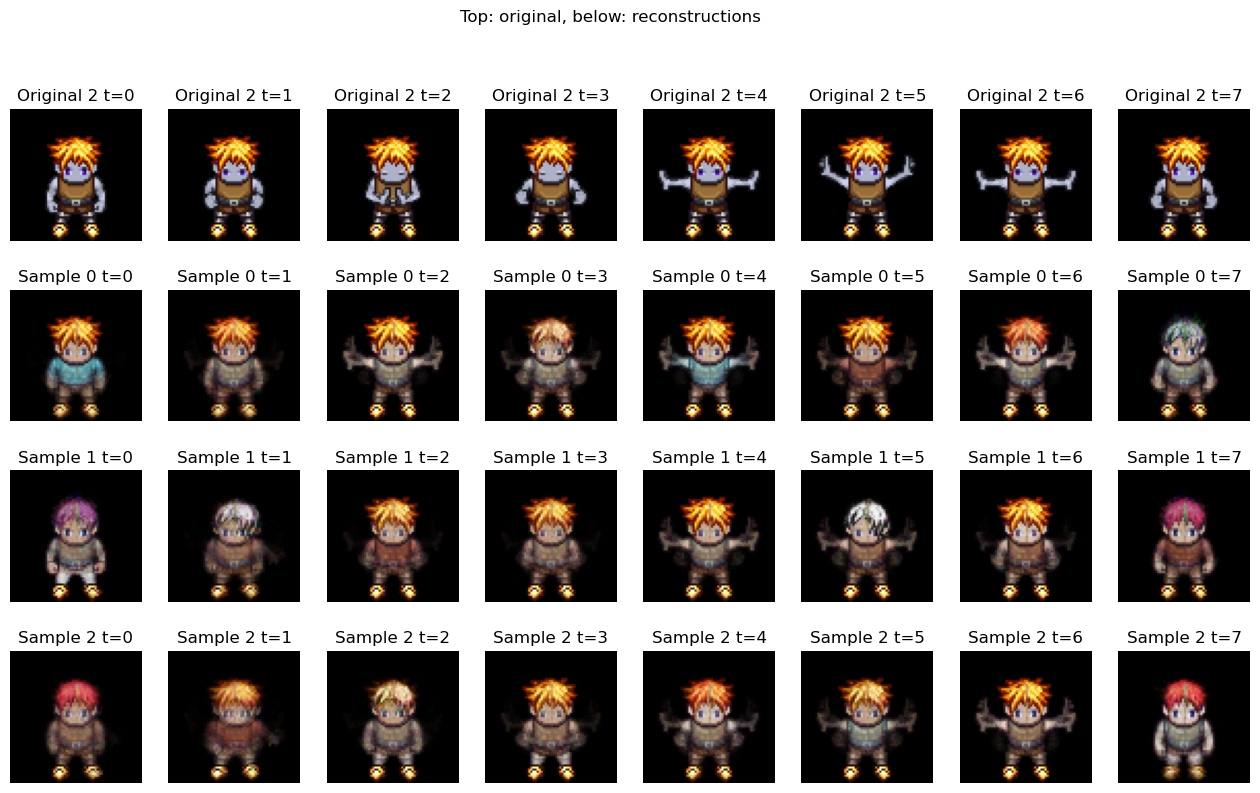
\includegraphics[width=0.7\textwidth]{/home/benjamin/Folders_Python/MVA/MVA_Stage/images/gpvae_reco_03.png}
    \caption{GPVAE Sprites reconstruction 3}
    \label{fig:GPVAE Sprites reconstruction 3}
\end{figure}
\end{frame}

\begin{frame}{GPVAE - Generation}
    \begin{figure}[H]
        \centering
        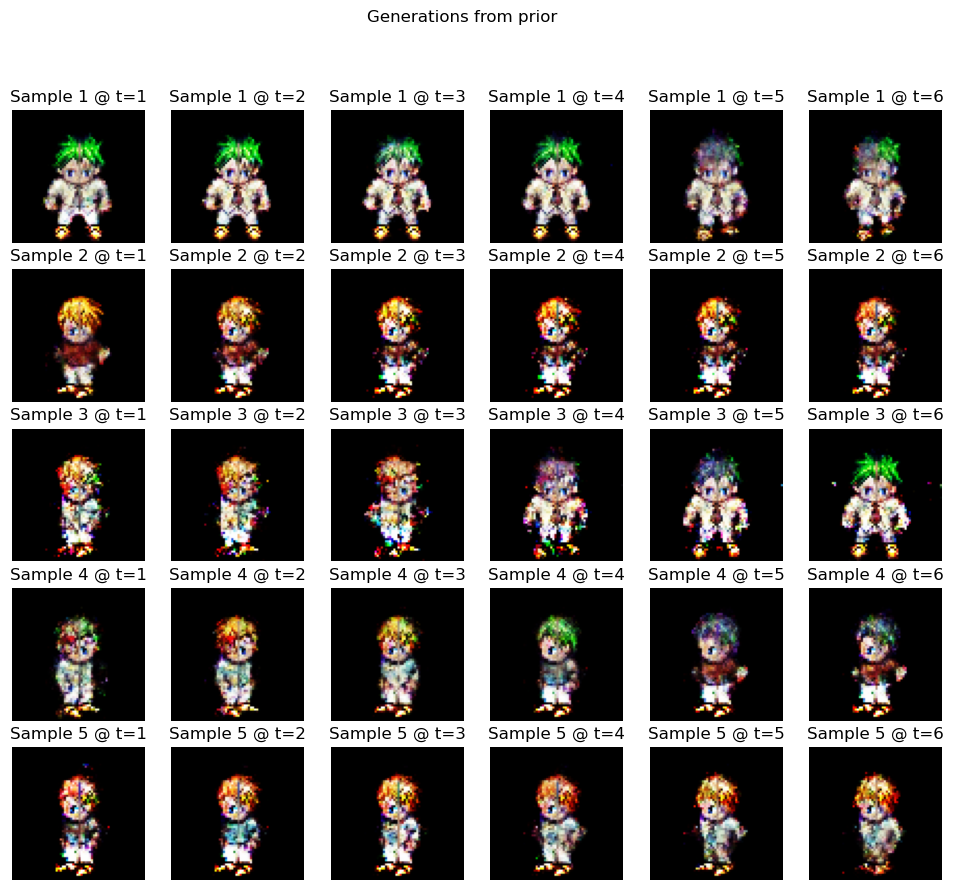
\includegraphics[width=0.45\textwidth]{/home/benjamin/Folders_Python/MVA/MVA_Stage/images/gpvae_gen_01.png}
        \caption{GPVAE Sprites generation 1}
        \label{fig:GPVAE Sprites generation 1}
    \end{figure}
\end{frame}
